\chapter{Discussion}
This chapter discusses the challenges, processes and decisions throughout the research. The main topics is the thesis' answer to the research questions. Further, the limitation of \gls{Wi-Fi} scope, how the events were triggered, why human analysis was selected and the reason to exclude the complexity of eavesdropping. 

\section{Our Answer to Research Question 1}
\textbf{Which private information can be gathered from a robot vacuum cleaner by carrying out a passive sniffing attack in a smart environment?}

It is possible to identify the presence of an Irobot Roomba i7 vacuum cleaner inside a smart environment based on the \gls{WLAN} or \gls{LAN} capture itself. In \gls{WLAN}, an attacker can eavesdrop and lookup all  \gls{MAC} addresses against open source registers. For \gls{LAN} capture the presence of \gls{DNS} requests to any Irobot owned domain will place a device behind the \gls{WAN} address.

The signature detection algorithm proposed and evaluated in this project was able to identify and attribute different events conducted on the Irobot Roomba i7. Detection of \textit{Automated cleaning} exposed information of when the user left the location, revealing private information. By observing the last five \textit{Automated cleaning} events in \textbf{Oslo} is was possible to identify when the user left work, collecting and analysis of events triggering over a longer time period can expose user behaviour. \textit{Application triggered cleaning} and \textit{Application start} was also identified exposing user interaction with the Irobot Roomba.

If implementations to differentiate physical triggered and scheduled cleaning are added, the detection of physical triggered cleaning will reveal user activity inside the smart environment. Schedule cleaning on the other hand can give away user routines. We can assume that users usually configure scheduled cleaning when there is a high probability that there is no one at the location. This can reveal environment routines. 

For \textit{Application triggered cleaning} and \textit{Application start} it is harder to identify the actual privacy exposure. The identification of these events can reveal more information if observed during longer time periods. Then user patterns and behaviors can be exposed. Users could trigger cleaning every time they are leaving for work or the gym.

As mentioned for \gls{WLAN} capturing, an attacker can extract private information as soon as the capturing is started because identification of the traffic is based in \gls{MAC} addresses. For \gls{LAN}, an attacker will have to eavesdrop \gls{WAN} traffic for up to 24 hours before the \gls{DNS} request to \textit{a2uowfjvhio0fa.iot.us-east-1.amazonaws.com} is sent, and the corresponding Irobot cloud service is identified. 

\section{Our Answer to Research Question  2}
\textbf{How can information exposed by the eavesdropping be misused by an attacker?} 

Private information exposed in an attack can be utilized to identify user behavior and routines. This could potentially reveal habits of when the user is leaving the environment, and identify user presence with high confidence. This information can be used to target user environment during empty hours, or address the environment when the user is present. Such information can also be sold to other actors. 

The identification of devices can be used  to target attacks, based on \gls{IoT} inventory. Spear phishing \cite{spear_phishing} will be more effective. They can also target attacks to exploit known or unknown vulnerabilities for the identified devices. This will increase the success rate of an attack. Exposed privacy information will threaten the security of any smart environment. 

\section{Our Answer to Research Question  3}
\textbf{Which security measures can be implemented to limit the exposed data and decrease the risk of misuse?} 

The most efficient way to defend against the detection algorithm, would be to implement traffic shaping. This could disrupt the predicted network traffic flows, pad existing packets or inject packets to break the patterns. This will be an effective way to defend against this in \gls{LAN} or \gls{WLAN} eavesdropping. A disadvantage with traffic shaping, will be higher latency and more data processing on local equipment. Implementation of traffic shaping could be on the robot vacuum cleaner itself, this would secure the communication regardless of the smart home environment infrastructure. Another approach is to implement this as a service within the smart environment, then the overall security of the smart environment would increase. 

Irobot should implement random \gls{MAC} addressing \cite{random_mac_bernardos2020rfc} for \gls{WLAN} communication. This would allow the Irobot vacuum cleaner to use a random \gls{MAC} address each time is connects to a new network, or change randomly to mislead an attacker. 

As for \gls{WAN} or \gls{LAN} traffic, \gls{DNS} is an easy identifier due to the use of \gls{Wi-Fi} channel encryption. The initial session needs to be established based on a \gls{DNS} request revealing the the \gls{IP} address to the initial corresponding host. However, the daily change of corresponding host could be communicated through the secure connection hiding the change in cloud server host. This would make the detection of Irobot Roomba traffic harder to conduct by an attacker.

\section{Collection of Wi-Fi Traffic}
The selected TP-Link \gls{AP} had \gls{IGMP} \cite{igmp_rfc2236} default enabled. This protocol enables devices on a local network to subscribe to different multicast groups. Return traffic will then be addressed to the multicast group and not the device's \gls{MAC} address. Due to this functionality, only the outbound traffic generated form the robot vacuum cleaner was captured during the standby event. Initial analysis of the standby traffic verified this when \gls{WLAN} basefilter was applied. These findings are shown in Figure \ref{fig:WLANIGMP_enabled}.

\begin{figure}[H]
    \centering
    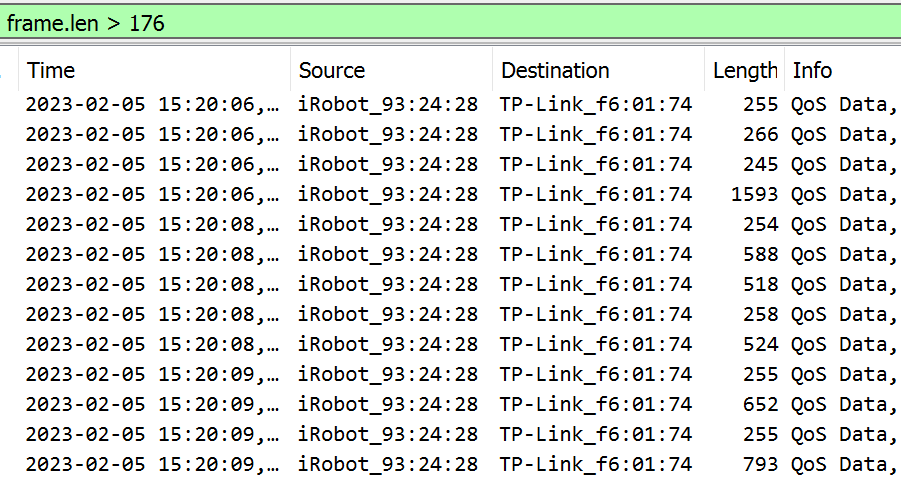
\includegraphics[width=0.8\textwidth]{figures/WLAN_IGMP_enabled.png}
    \caption{Wireshark \gls{WLAN} capture, included basefilter and enabled IGMP}
    \label{fig:WLANIGMP_enabled}
\end{figure}

If \gls{IGMP} enabled \gls{Wi-Fi} would to be in the scope of this thesis, a process of filtering based on multicast group addresses should have been implemented. A 20 minutes \textit{Application triggered cleaning} capturing was conducted in \textbf{Oslo} capturing only traffic including the \gls{MAC} address of the AP. The capture included 9,342 packets, which is 340\% more than \gls{LAN} traffic average for the same event. By applying a Wireshark filter, excluding all traffic except Irobot and multicast \gls{MAC} addressed, we identified the new \gls{IGMP} traffic flow, shown in Figure \ref{fig:WLANIGMP_all_enabled}. 

\begin{figure}[H]
    \centering
    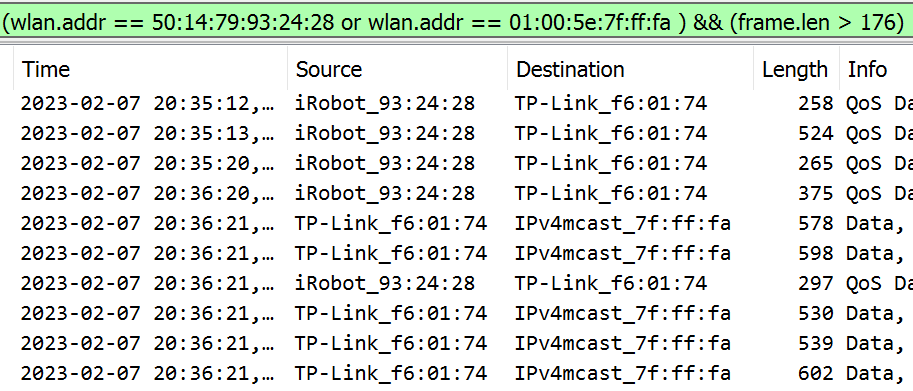
\includegraphics[width=\textwidth]{figures/WLAN_IGMP_ALL.png}
    \caption{\gls{WLAN} IGMP application triggered cleaning test in Oslo}
    \label{fig:WLANIGMP_all_enabled}
\end{figure}

This increases the complexity of the filtering mechanisms and identification of multicast traffic in \textbf{Oslo} and \textbf{Drammen}. The complexity occurs when more then one \gls{IoT} device is connected to the same network. Devices can subscribe to the same or a new multicast group making the wireless environment more complex and hard to navigate in. \gls{IGMP} is not used in all \gls{Wi-Fi} networks \cite{wifi_ieee80211} and it is therefor disabled on the AP. 

\section{Event Triggering}
As shown in Chapter \ref{cap:AnalysisandResults}, several events were triggered during the same day and with limited time between them. The reason for this is the time constraint of this master project and the availability of smart environments. This increases the possibility of cross event influence, especially in the end of cleaning when the Irobot Roomba uploads cleaning data to the cloud service at \textit{s3.amazonsaws.com}. To mitigate the influence, it was decided to only focus on the event initiation and not the end of cleaning reporting. Event triggering traffic is assumed to be the same regardless of previous events. 

Real-life simulation of a smart environment is hard to recreate as there will not be triggered 5 cleaning events, within 2 hours. Event triggering timestamps in this project will appear unrealistic due to structured triggering in a short time period. Timestamps captured and identified in this research can therefore not be used in attributing events, but as mentioned in the analysis it could be a good attribute to include in the analysis and extraction of user private information.  

\section{Method of Analysis}
Both human-based analysis and machine learning were discussed as the traffic analysis method in this project. Several other researches have used machine learning to extract information from network traffic based on various attributes. During the literature review no documentation describing Irobot Roomba's communication pattern or protocols was found, Irobot did also not reply with information upon requests for this information. Either way, the data would have to be pre-processed by a human to identify which attributes that could be used in further analysis. The analysis method was therefore decided to be manual human-learn rule-based learning. 

\section{The Complexity of Eavesdropping}
The level of complexity of conducting an eavesdropping attack for \gls{WLAN}, \gls{LAN} or \gls{WAN} is not addressed in this thesis. This is a topic which should be addressed in separate research, due to the variety of devices and configurations in different smart environments. Smart environments used in this project only serve Internet access to exclude possible local configuration. 

In wireless eavesdropping, an attacker would only need to be in wireless range of the targeted devices to collect corresponding network traffic. Eavesdropping devices can be placed in the vicinity of the smart environment or installed inside an environment, collected data can be stored locally or exported to a online service through Internet connection. There are pros and cons with the different approaches which is not addressed. For \gls{LAN} and \gls{WAN} eavesdropping the attacker would need physical access to the local network, or exploit remote access to network devices. These operations challenge both physical and technical security and are therefore out of scope for this thesis. 



